%! Author = Philipp Emmenegger
%! Date = 09/06/2021

\subsection{Factory Method}
Define an interface for creating an object, but let subclasses decide which class to instantiate.\\
Factory Method lets a class defer instantiation to subclasses.\\
\begin{itemize}
    \item Can be \textit{abstract} or \textit{virtual}
    \item Can be parameterized
    \item Typically called from within a Template Method
    \item Names start with \textit{Create}-prefix
\end{itemize}

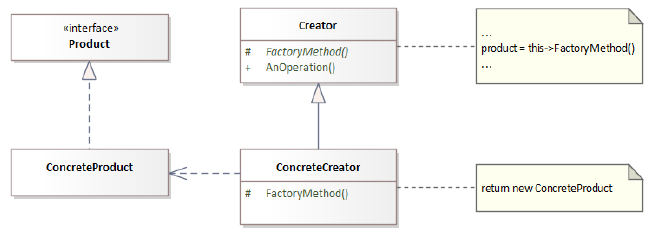
\includegraphics[width=\linewidth]{../img/factory_method.png}
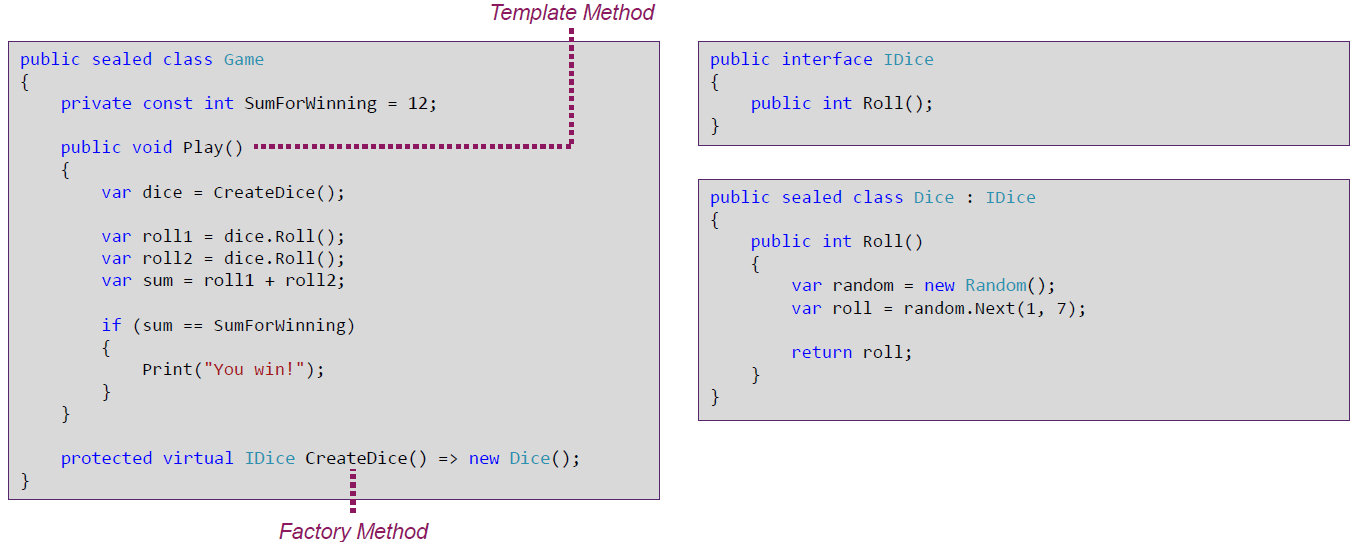
\includegraphics[width=\linewidth]{../img/factory_method_code.png}

\subsection{Abstract Factory}
Provide an interface for creating families of related or dependent objects without specifying their concrete classes.\\
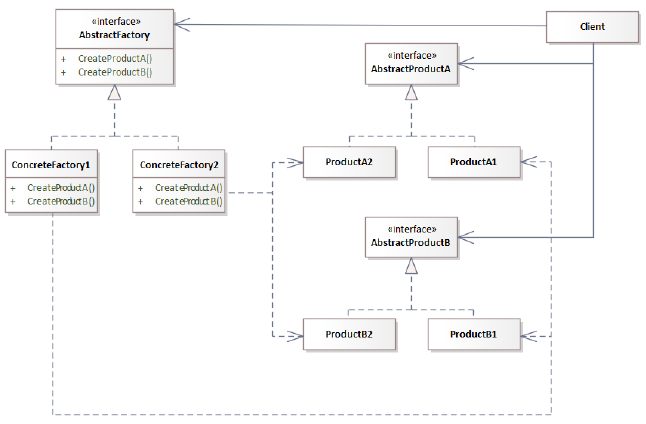
\includegraphics[width=\linewidth]{../img/abstract_factory.png}
\begin{itemize}
    \item Composition should be favored over inheritance
    \item Object creation is a responsibility - can justify a seperate class (SRP)
    \item Move object creation to a class called Factory
    \item Inject an object of that factory into the Game
\end{itemize}
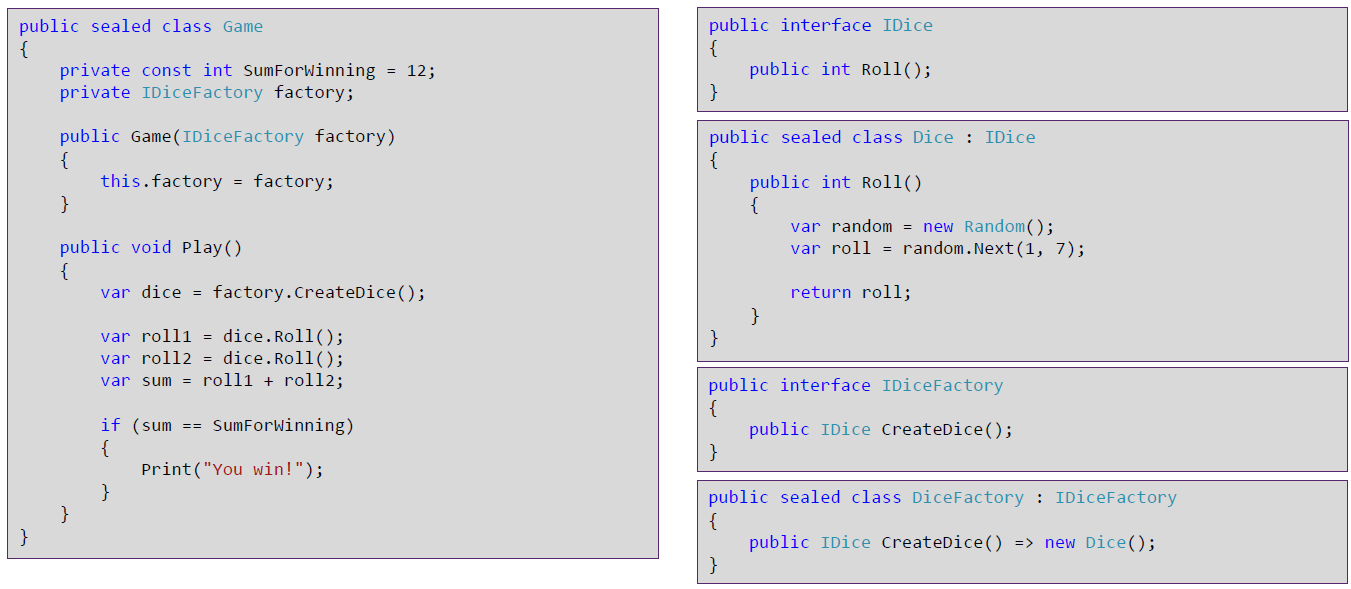
\includegraphics[width=\linewidth]{../img/abstract_factory_code.pong.png}

\subsection{(Simple) Factory}
\begin{itemize}
    \item Strategy for creating objects
    \item Creating objects with hardcoded values
    \item Creating objects read from a database
    \item Creating objects read from a webservice
\end{itemize}
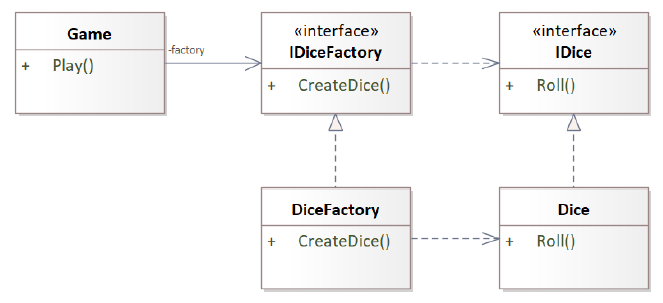
\includegraphics[width=0.7\linewidth]{../img/factory_pattern.png}

\subsection{Singleton}
Ensure a class only has one instance, and provice a global point of access to it.\\
\textbf{Drawbacks:}
\begin{itemize}
    \item Globals with high coupling
    \item Hard to test
    \item Error-prone when multi-threading
\end{itemize}
\textbf{If you need a single instance:}
\begin{itemize}
    \item Create it in your main and inject it
    \item Let a Factory or Proxy manage its lifecycle
\end{itemize}
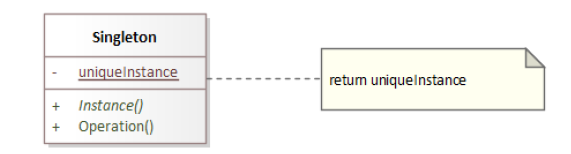
\includegraphics[width=0.7\linewidth]{../img/singleton_pattern.png}\\
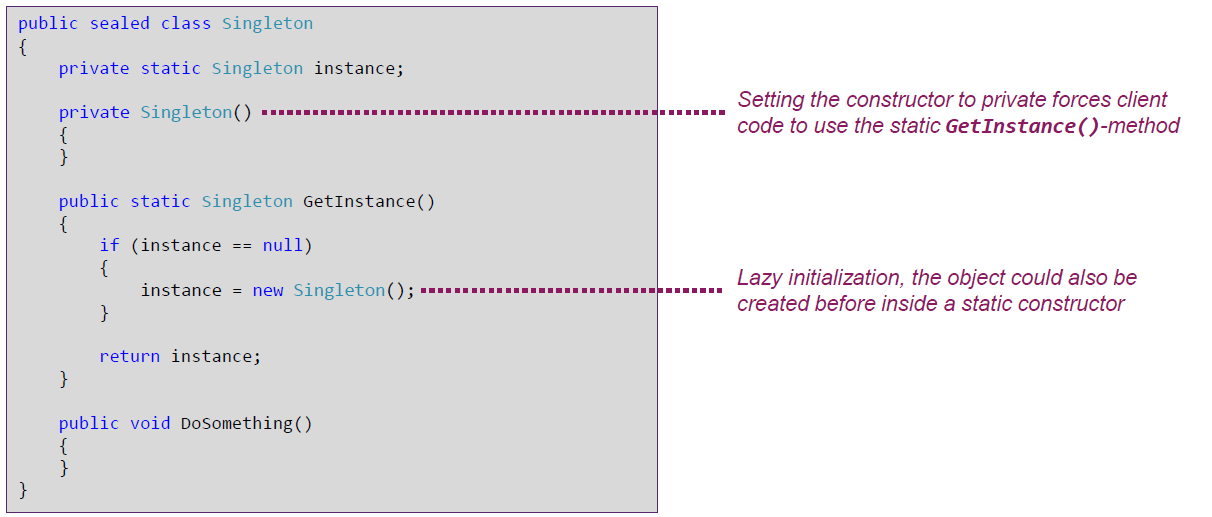
\includegraphics[width=\linewidth]{../img/singleton_pattern_code.png}

\subsection{Adaper}
Convert the interface of a class into another interface clients expect.\\
Adapter lets classes work together that couldn't otherwise because of incompatible interfaces.\\
\begin{itemize}
    \item Adapter can add functionality to Adaptee
    \item If creating the Adaptee is complex, think about Injection or Factories
\end{itemize}
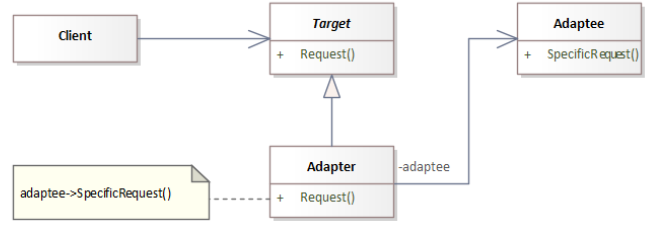
\includegraphics[width=0.7\linewidth]{../img/adapter_pattern.png}\\
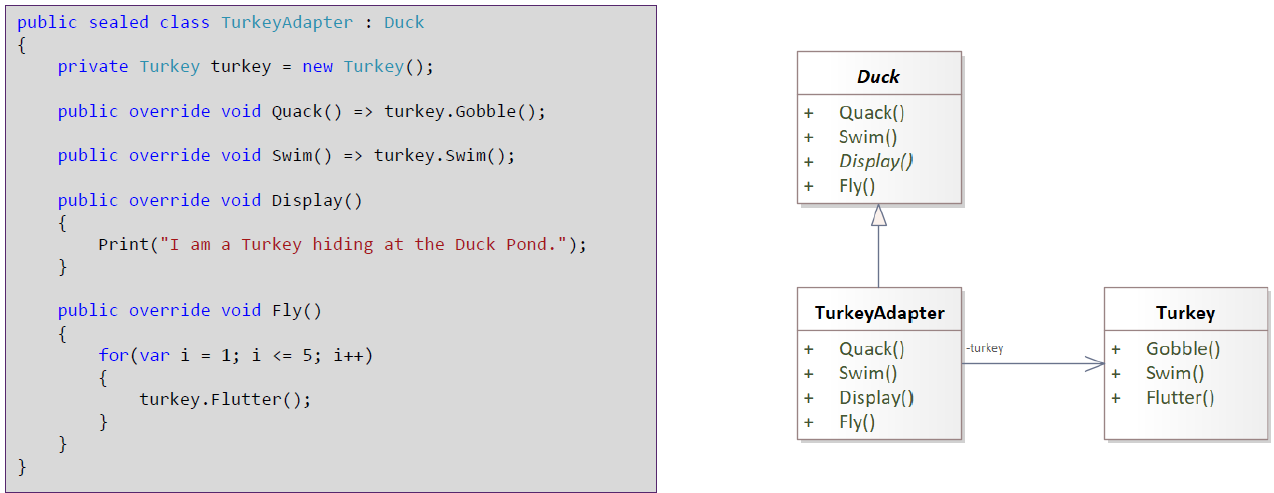
\includegraphics[width=\linewidth]{../img/adapter_pattern_code.png}\\
\subsubsection{Variants}
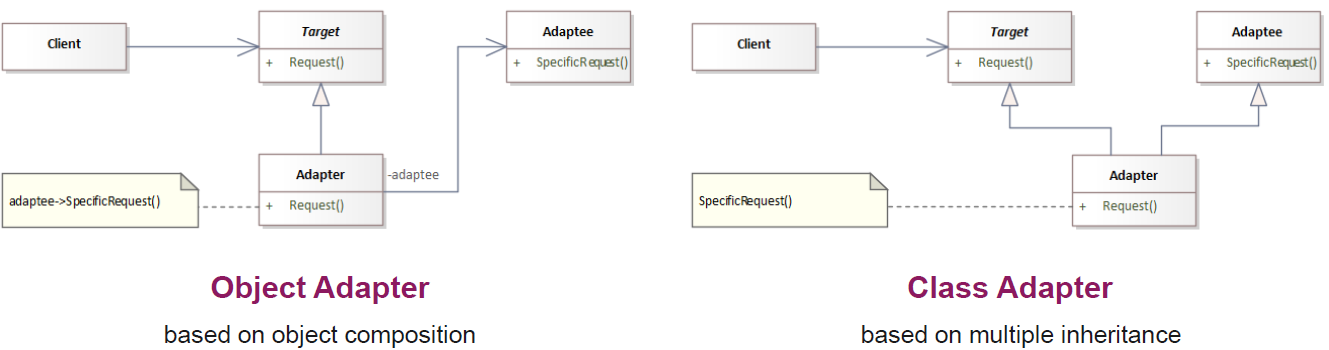
\includegraphics[width=\linewidth]{../img/adapter_pattern_variants.png}

\subsection{Facade}
Provide a unified interface to a set of interfaces in a subsystem.\\
Facade defines a higher-level interface that makes the subsystem easier to use.\\
\begin{itemize}
    \item Decouples a client from a complex, internal / external subsystem
    \item Keep the interface of the Facade small
    \item Multiple Facades for the same subsystem possible (SRP)
    \item Helps to achieve exchangeability
\end{itemize}
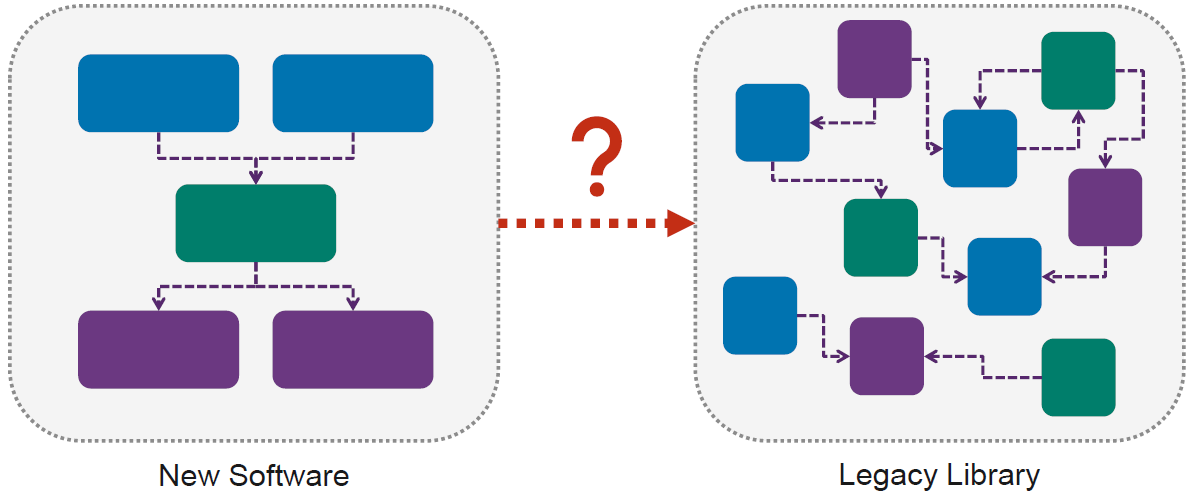
\includegraphics[width=\linewidth]{../img/facade_pattern.png}

\subsection{Composite}
Compose objects into tree structures to represent part-whole hierarchies.\\
Conposite lets clients treat individual objects and compositions of objects uniformly.\\
\begin{itemize}
    \item Trade off between SRP and transparency
    \item Component as interface / abstract class possible
    \item Component with abstract or virtual methods possible
\end{itemize}
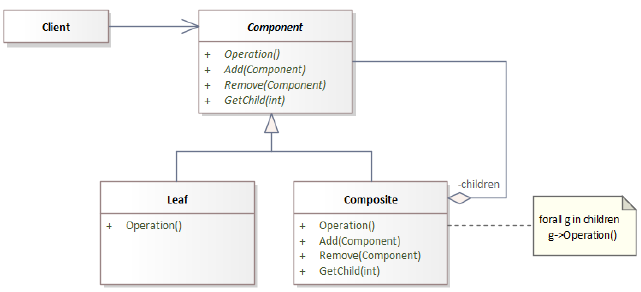
\includegraphics[width=0.7\linewidth]{../img/composite_pattern.png}\\
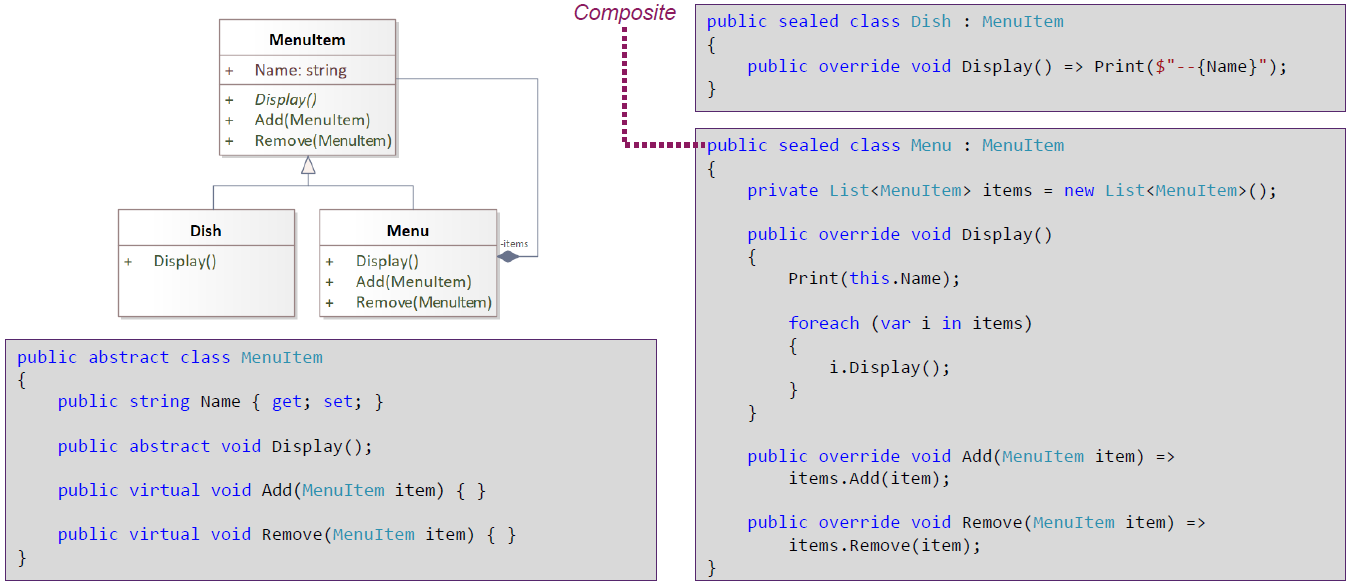
\includegraphics[width=\linewidth]{../img/composite_pattern_code.png}\\
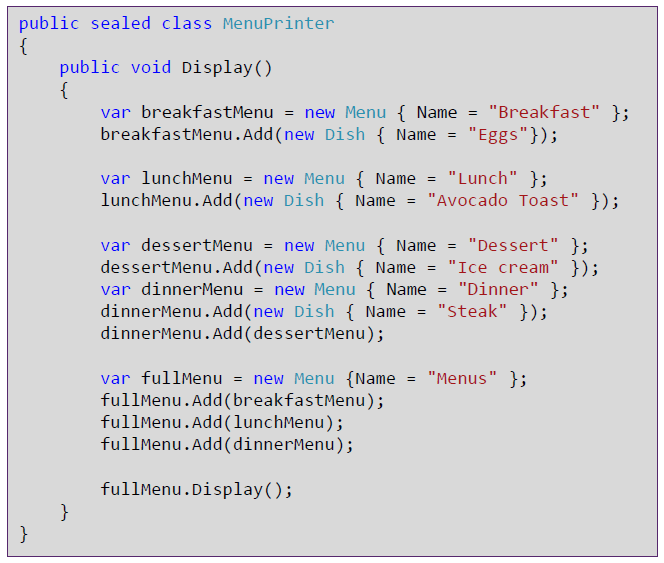
\includegraphics[width=0.7\linewidth]{../img/composite_pattern_code_2.png}\\

\subsection{Decorator}
Attach additional responsibilites to an object dynamically.\\
Decorators provide a flexible alternative to subclassing for extending functionality.\\
\begin{itemize}
    \item Alternative to subclassing for extending behaviour
    \item Added behaviour before/after method calls to component
    \item Transparent to the client
    \item Decorator: change the skin of object
    \item Strategy: change the guts
\end{itemize}
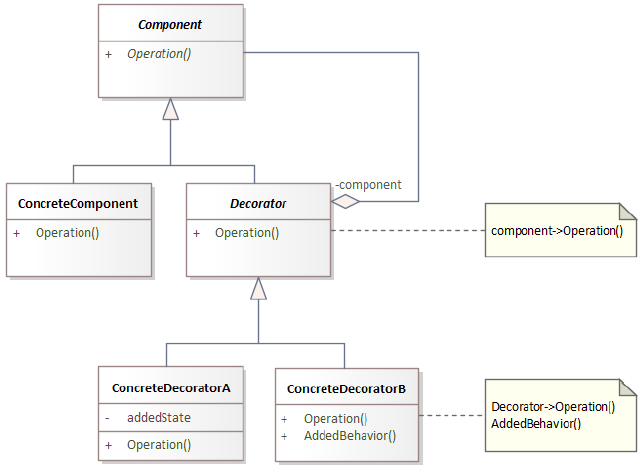
\includegraphics[width=0.8\linewidth]{../img/decorator_pattern.png}\\
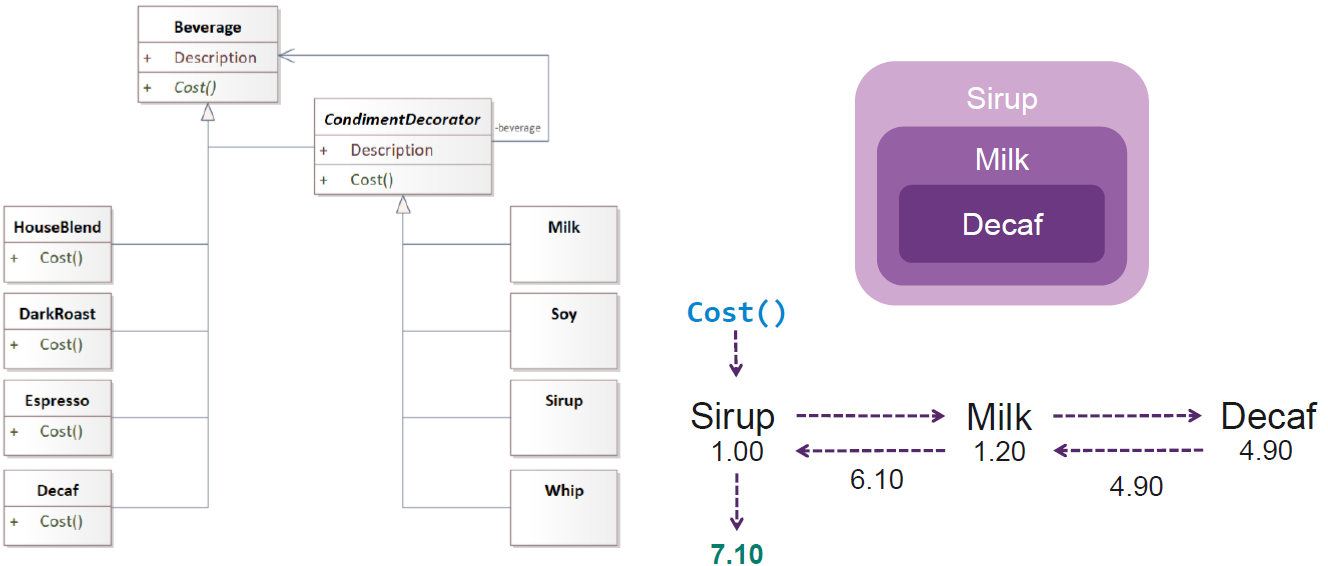
\includegraphics[width=\linewidth]{../img/decorator_pattern_2.png}\\
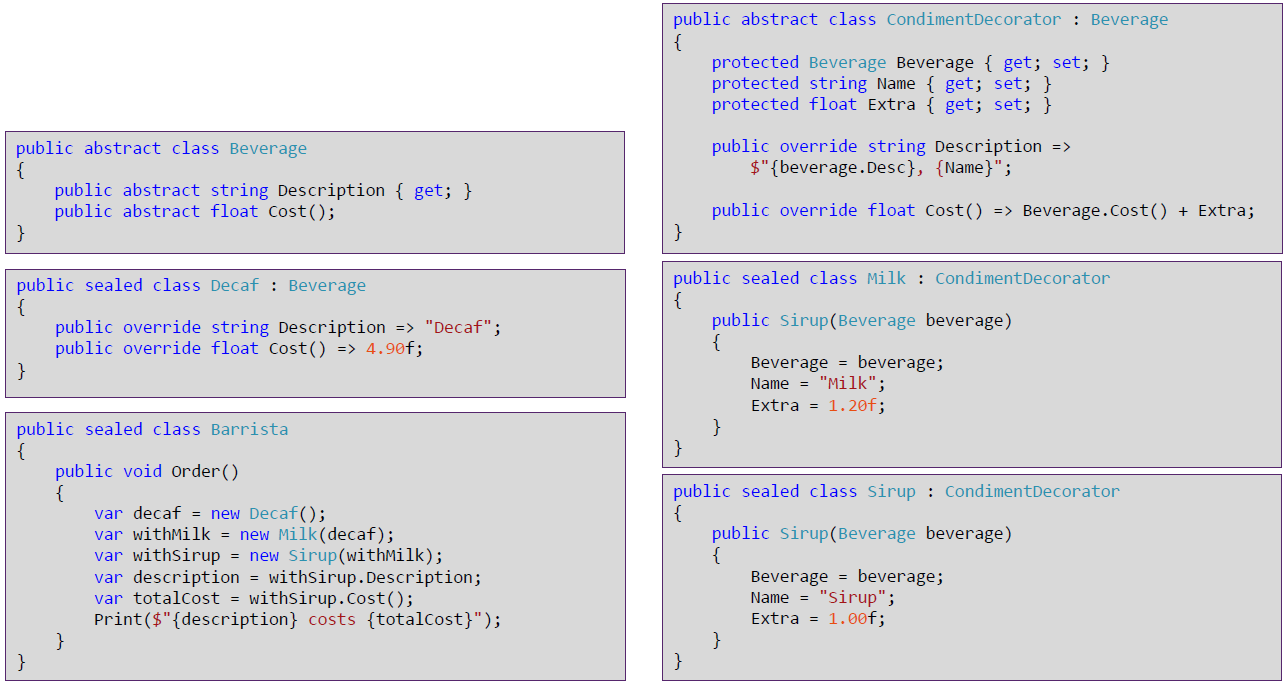
\includegraphics[width=\linewidth]{../img/decorator_pattern_code.png}\\

\subsection{Proxy}
Provide a surrogate or placeholder for another object to control access to it.\\
\begin{itemize}
    \item Often created within a Factory
    \item Controls access to the wrapped object
    \item Proxy and wrappee have the same interface
\end{itemize}
\textbf{Variations}
\begin{itemize}
    \item Virtual Proxy: access to an expensive to instantiate object
    \item Remote Proxy: interaction between a client and a remote object
    \item Protection Proxy: controls access to the original object
\end{itemize}
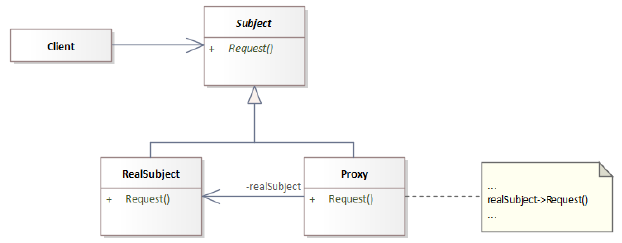
\includegraphics[width=0.8\linewidth]{../img/proxy_pattern.png}
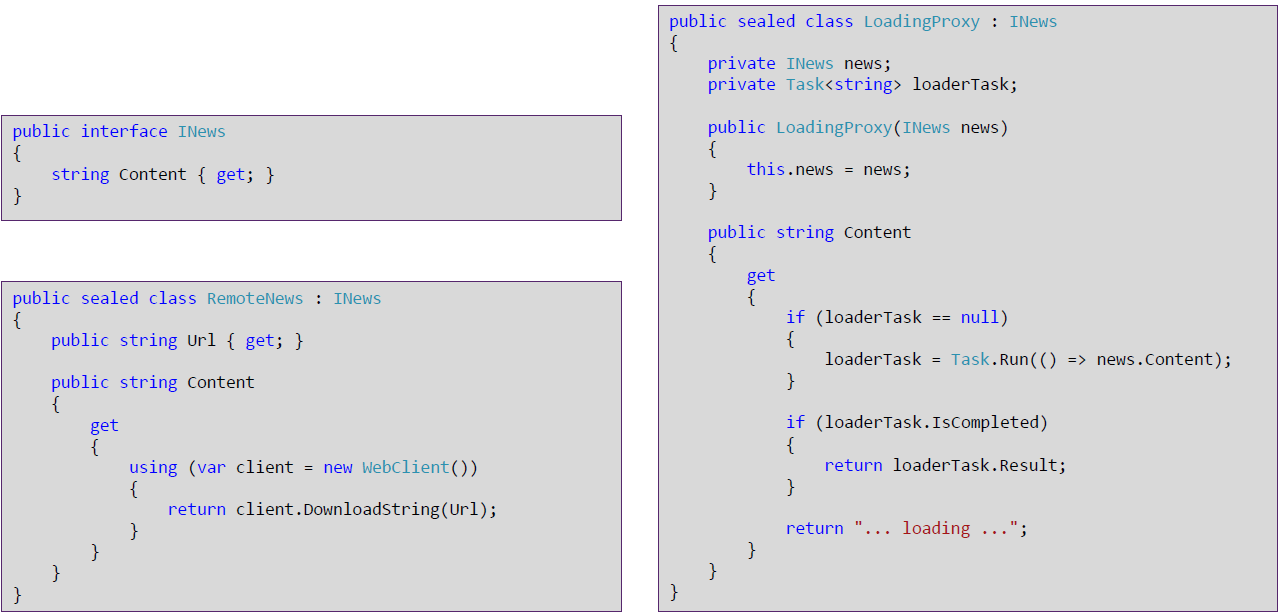
\includegraphics[width=\linewidth]{../img/proxy_pattern_code.png}

\subsection{Summary}
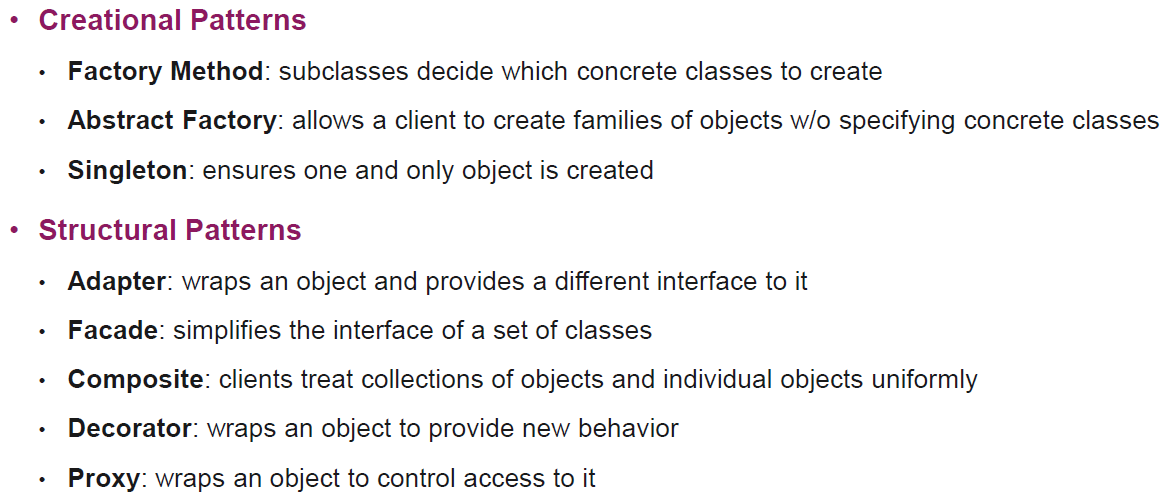
\includegraphics[width=\linewidth]{../img/patterns_summary.png}


